\section{Noise compounds super-additively}
\label{sec:noise}

We injected depolarising error on one- and two-qubit gates and readout error,
first individually and then factorially. Individually, none of the three is
distinguishable from no noise at all, even at $30\%$ error
(Fig.~\ref{fig:logistic}).

Factorially they compound, and they compound \emph{more than independently}.
Table~\ref{tab:noise} crosses two-qubit and readout error at three levels
each. The observed success rate exceeds --- in the sense of falling below in
success, hence exceeding in damage --- the rate an independence assumption
would predict in \textbf{all nine cells}, by between $4.7$ and $9.9$
percentage points. The worst cell, both channels high, succeeds $81.5\%$ of
the time.

\begin{table}[htbp]
\centering\small
\caption{Factorial noise interaction, two-qubit depolarising against
readout error, 27 trials per cell. ``Independence'' is the success rate
predicted by treating the two channels as acting independently at their
measured single-source rates; ``excess'' is the shortfall of the observed
rate against it. Every cell is positive, so the channels compound
super-additively. From \texttt{phase2\_noise\_combined.csv}.}
\label{tab:noise}
\begin{tabular}{@{}llrrr@{}}
\toprule
2-qubit & Readout & Observed & Independence & Excess \\
\midrule
none & none & 0.963 & 0.892 & $+0.071$ \\
none & med  & 0.926 & 0.857 & $+0.069$ \\
none & high & 0.926 & 0.834 & $+0.092$ \\
med  & none & 1.000 & 0.904 & $+0.096$ \\
med  & med  & 0.926 & 0.868 & $+0.057$ \\
med  & high & 0.926 & 0.845 & $+0.081$ \\
high & none & 0.889 & 0.822 & $+0.067$ \\
high & med  & 0.889 & 0.790 & $+0.099$ \\
\textbf{high} & \textbf{high} & \textbf{0.815} & 0.768 & $+0.047$ \\
\bottomrule
\end{tabular}
\end{table}

\begin{figure}[htbp]
\centering
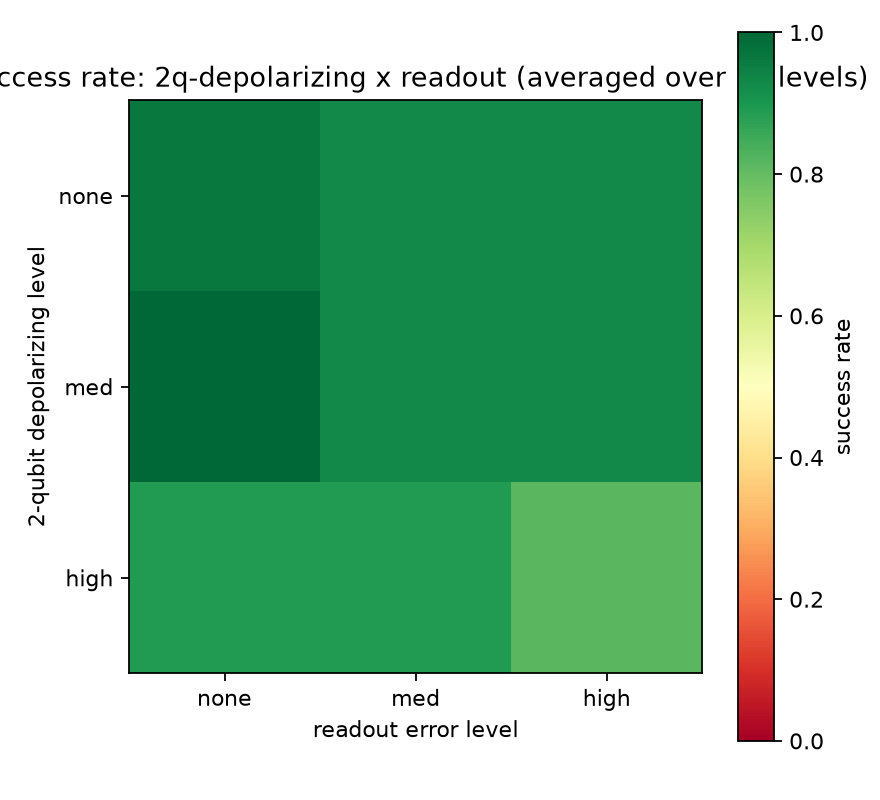
\includegraphics[width=0.72\linewidth]{../Data/failure_study/plots/noise_combined_heatmap.png}
\caption{\textbf{Success rate across the factorial noise grid.} The gradient
runs diagonally: neither channel alone moves the outcome much, and their
combination does. Rendered from \texttt{phase2\_noise\_combined.csv}.}
\label{fig:noise}
\end{figure}
